\section{Evaluation}
\label{sec:evaluation}


%##########################################################
%                     SEC EValuation                      %
%##########################################################

In this section we analyze \ac{xctp} and compare it with three protocols: \ac{ctp}, \ac{rpl}, and \ac{aodv}. The objective of this analysis is to show that the protocol is working properly, as well as to evaluate \ac{xctp} performance when compared with the current state-of-the-art protocols. We analyzed according to
the following items:
\begin{inparaenum}
    \item favoring the construction of data transport protocols;
    \item robustness in the presence of faults in different topologies;
    \item scalability.
    \item control traffic.
\end{inparaenum}

%----------------------
% SUBSEC Simulation   %
%----------------------
\subsection{Simulation}
\label{sec:simulation}

Of the protocols shown in Table~\ref{tab:comp-paradigmas}, Directed Diffusion~\cite{directedDiffusion}, Deluge~\cite{deluge}, (DIP, DRIP, DHV)~\cite{tinyos} are used just for data dissemination in the network and do not serve to compared with \ac{xctp}. \acf{ctp}~\cite{ctp} is one of the newest protocols and it presents better results than MultiHopLQI~\cite{MultiHopLQI} and MintRoute~\cite{mintroute} in data collection. To the best of our knowledge, there are no stable and open source implementations to the community of Dymo~\cite{dymo}, \ac{dsr}~\cite{DSR} and Hydro~\cite{hydro}. Therefore, we made comparisons with \ac{rpl}~\cite{RPL}, \ac{aodv}~\cite{AODV}, and \ac{ctp}.

\ac{xctp}, \ac{ctp}, and \ac{aodv} were implemented in the TinyOS~\cite{tinyos}. We adopted \ac{rpl}
Contiki~\cite{contiki} implementation. We also performed experiments with Tymo, a TinyOS version of protocol Dymo. However, Tymo implementation did not show to be stable as reported in \cite{tymo}.

\begin{table}[!ht]
\normalsize
\caption{Simulation parameters}
\label{tab:param}
\centering

%\resizebox{\linewidth}{!}{%
\begin{tabular}{l|c}
\hline
\multicolumn{1}{c|}{\textbf{Parameter}} & \textbf{Value}  \\ \hline
Base station                            & $1$ center        \\
Number of sensors                       & $100$             \\
Radio range ($m$)                         & $100$          \\
Density ($nodes/m^2$)                   & $10$ \\
Number of experiments                   & $100$ \\
Bytes transmitted                       & $1024$ \\
Path Loss Exponent                      & $4.7$\\
Power decay ($dB$)                        & $55.4$\\
Shadowing Std Dev ($dB$)       			& $3.2$\\
\end{tabular}
%}

\end{table}

We run the experiments on the simulator for \ac{l2ns} TOSSIM~\cite{tossim}. We consider the base station to be a PC without memory restrictions and which can hold information about the entire network topology. we used the LinkLayerModel tool from TinyOS to generate the topology and connectivity model. We consider $10$ different topologies. In each scenario were runs $10$ simulations, totaling $100$ runs. In the graphs presented, the curve represents the average and the error bars is the confidence interval of $95\%$. Table~\ref{tab:param} presents the default simulation parameters.

%----------------------------
% SUBSEC Simulation Results %
%----------------------------

\subsection{Simulation Results}
\label{sec:simulation-results}

Figure~\ref{fig:delivery-512KB} shows the percentage of delivery of a file of size $512KB$ sent from the root to a sensor node $5$ hops away. \ac{xctp}+\ac{tp}, \ac{aodv}+\ac{tp}, and \ac{rpl}+\ac{tp} reach $100\%$ of data delivery, because they allow feedbacks to be sent from data received between the two involved in the communication. We observed that \ac{ctp} can transfer only $96.5\%$ of the $512KB$, because it is not possible to request lost data or confirm received messages, since there are routes only towards the root. The impossibility of requesting the remaining fragments results in malfunctioning the application that is intolerant to data loss. We conclude that \ac{xctp}, \ac{aodv}, and \ac{rpl}  favor the development of data transport protocols, providing routes that allow feedback messages to be exchanged among sensor nodes and the base station.

\begin{figure}[t]
\centerline{
    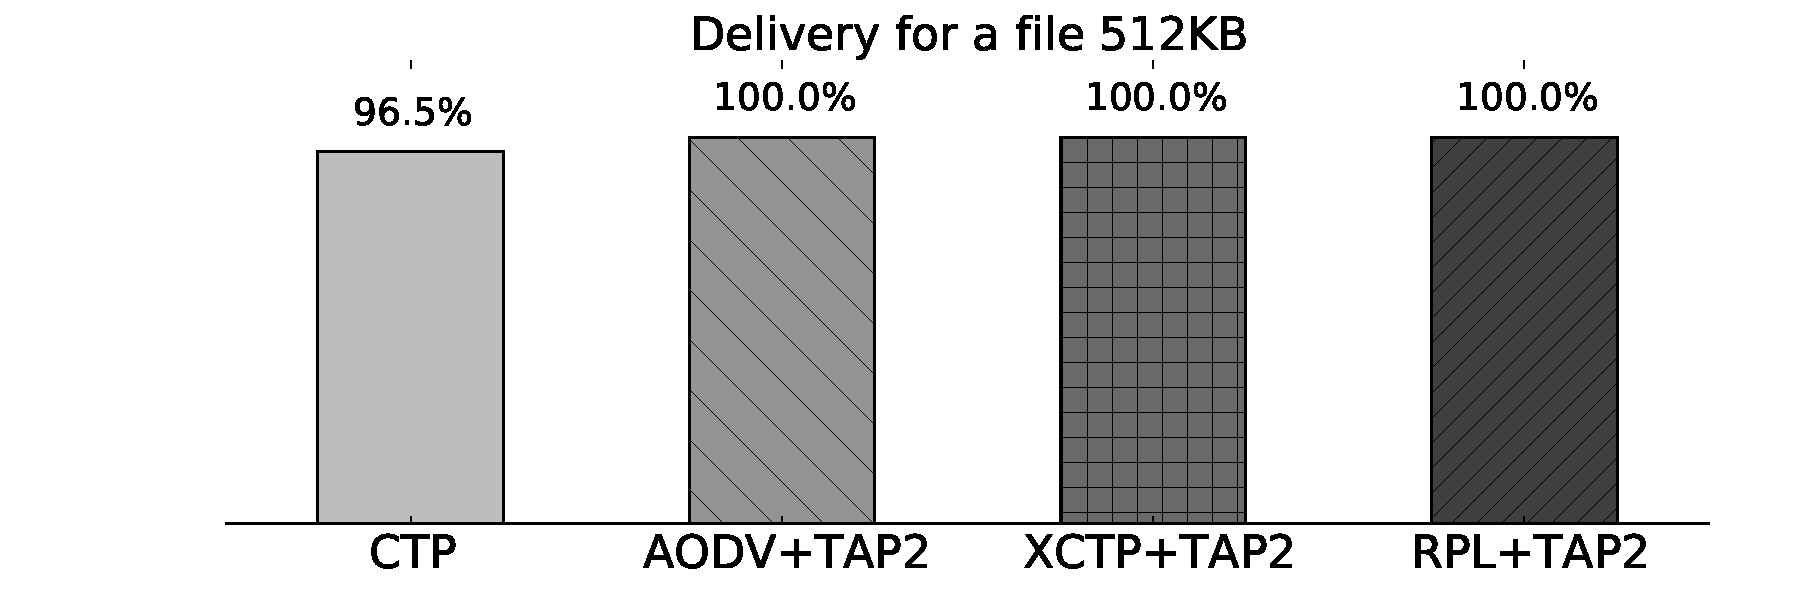
\includegraphics[width=0.8\linewidth]{img/entrega-512KB}
} \caption{Transferring a 512KB file to a node 5 hops away
from the root.} \label{fig:delivery-512KB}
\end{figure}

%--------------------
% SUBSEC Robustness %
%--------------------
\subsubsection{Robustness}
\label{sec:robustness}

To evaluate \ac{xctp} in terms of robustness, we elaborated experiments with different amounts of active flows (nodes transmitting data to root) and inserted network failures.

\begin{figure}[ht]
\centerline{
    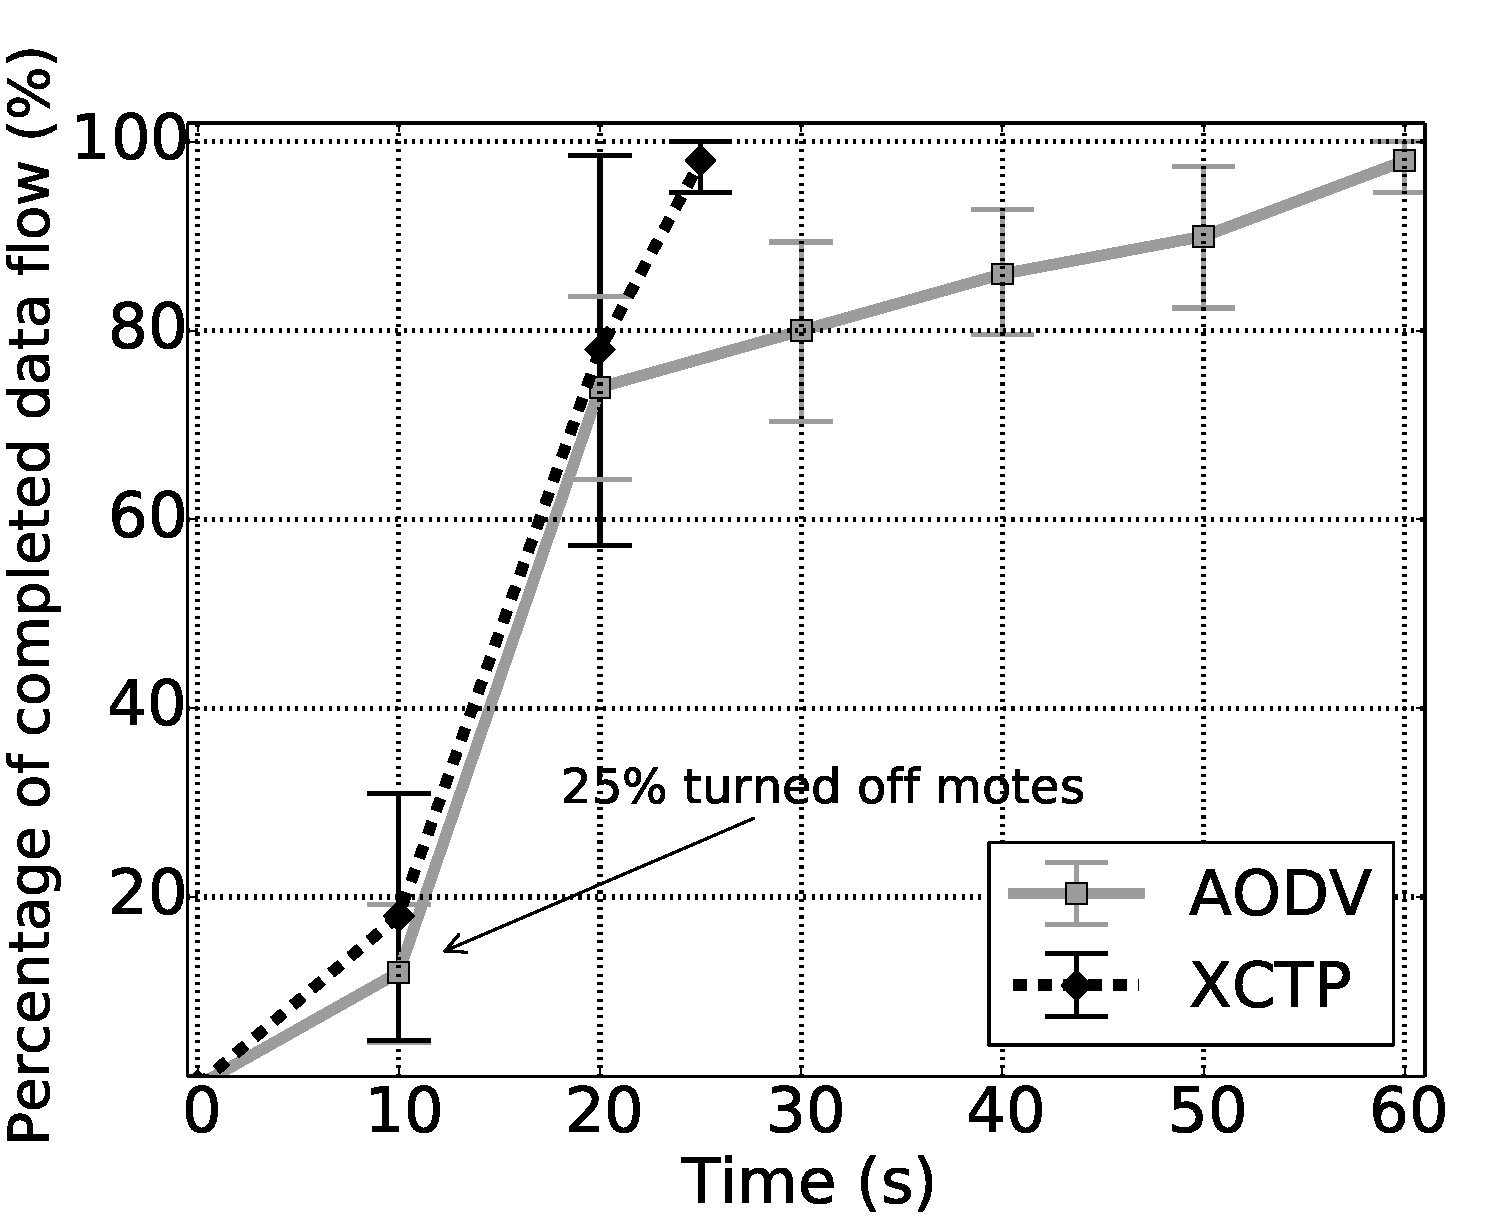
\includegraphics[width=0.55\linewidth]{img/reacao-xctp-vs-aodv-line2}
} \caption{\ac{xctp} and \ac{aodv} reactions in the occurrence of network failures.} \label{fig:reaction-aodv-vs-xctp}
\end{figure}

Initially we compared \ac{xctp} and \ac{aodv} with respect to the reaction in
the presence of network failures. In this scenario, $5$ sensor nodes transfer,
each one, $1KB$ of data to root reliably and after $10s$ from the beginning of
transmission we disable $25\%$ of the network, without creating disconnected
components in the network. Figure~\ref{fig:reaction-aodv-vs-xctp} shows in
y-axis the percentage of flows that have completed the transfer of $1KB$ of
data, the x-axis shows the elapsed time. In the first seconds of the simulation
the two approaches are similar, being \ac{xctp} a little faster due to
proactive construction of routes. After the shutdown of part of the network at
$10s$, \ac{xctp} reacts quickly finding new routes to the root, the $5$ sensor
nodes operating with \ac{xctp} complete the transfer in
approximately $25s$. \ac{aodv} reacts slowly to topological
change. \ac{aodv} on average takes $60s$ to complete all data transfers, in some scenarios, \ac{aodv} took over $200s$ to finish.

%\begin{figure}[!ht]
%\centerline{
%    \subfigure[fig:reaction-aodv-vs-xctp][\ac{xctp} and \ac{aodv} reactions in the occurrence of network failures.]{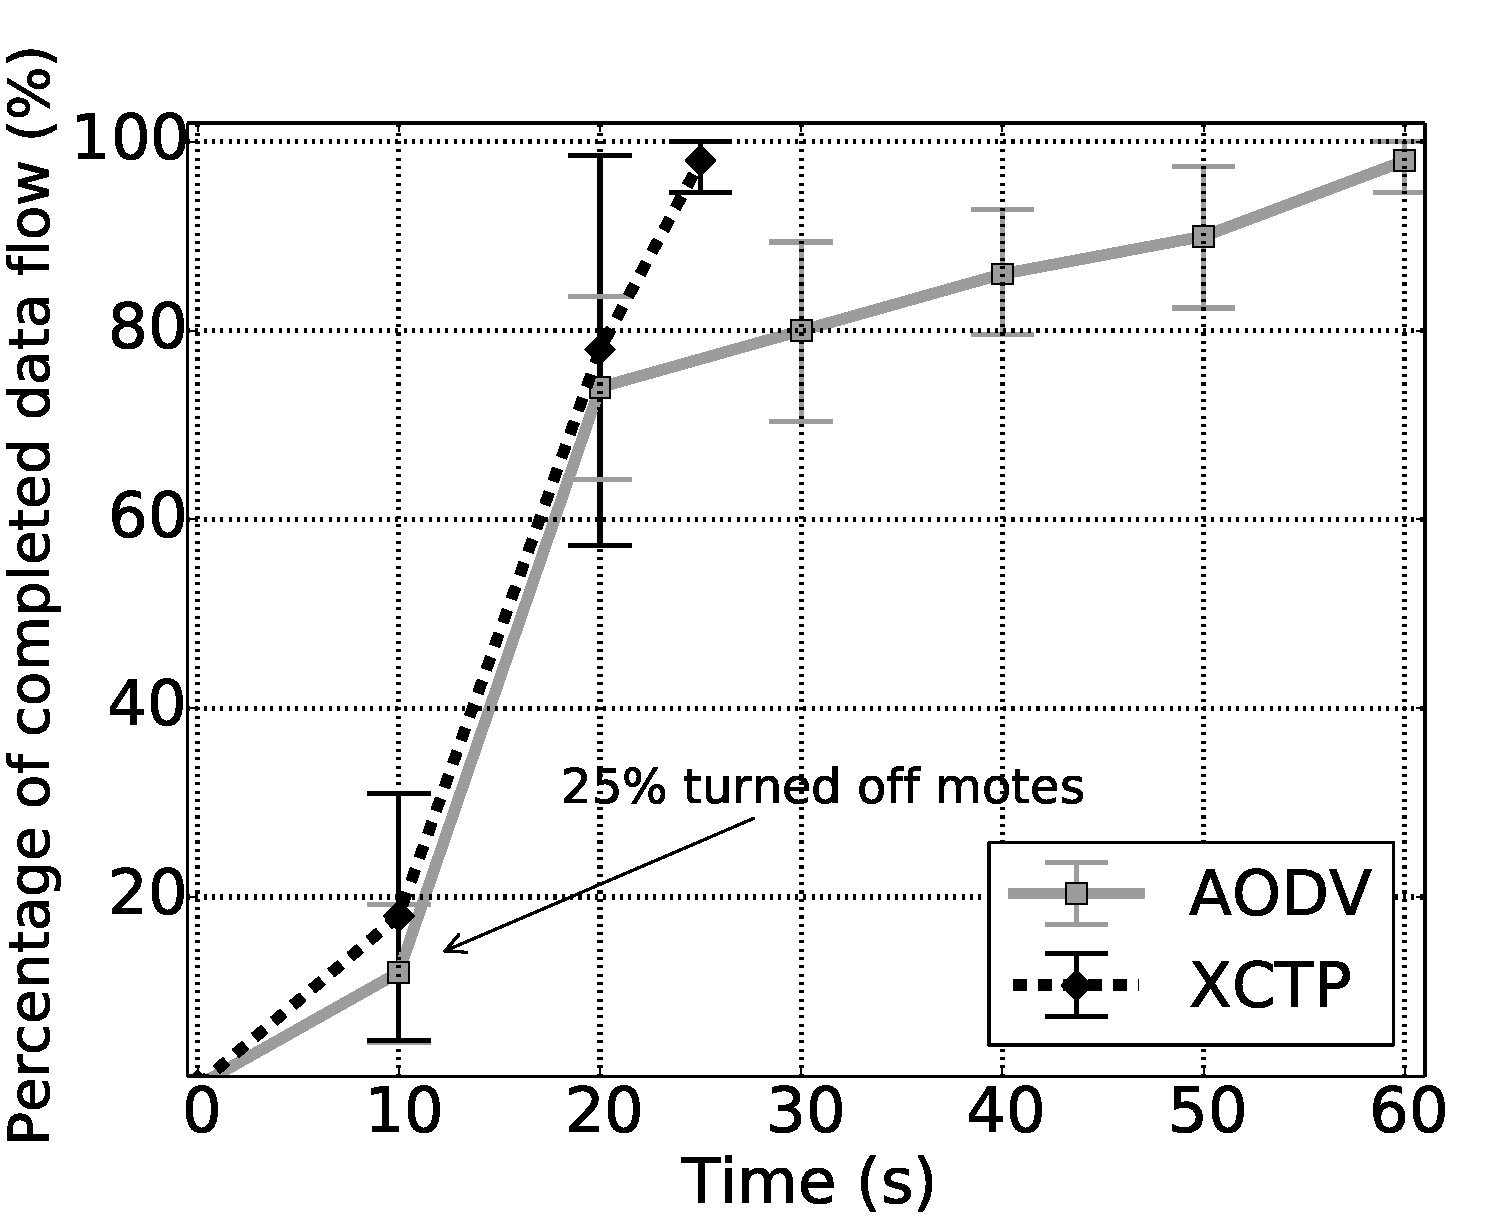
\includegraphics[width=0.47\linewidth]{img/reacao-xctp-vs-aodv-line2}\label{fig:reaction-aodv-vs-xctp}}
%\,
%    \subfigure[fig:reaction-xctp][\ac{xctp} reaction in the presence of failures. $50$ flows are active.]{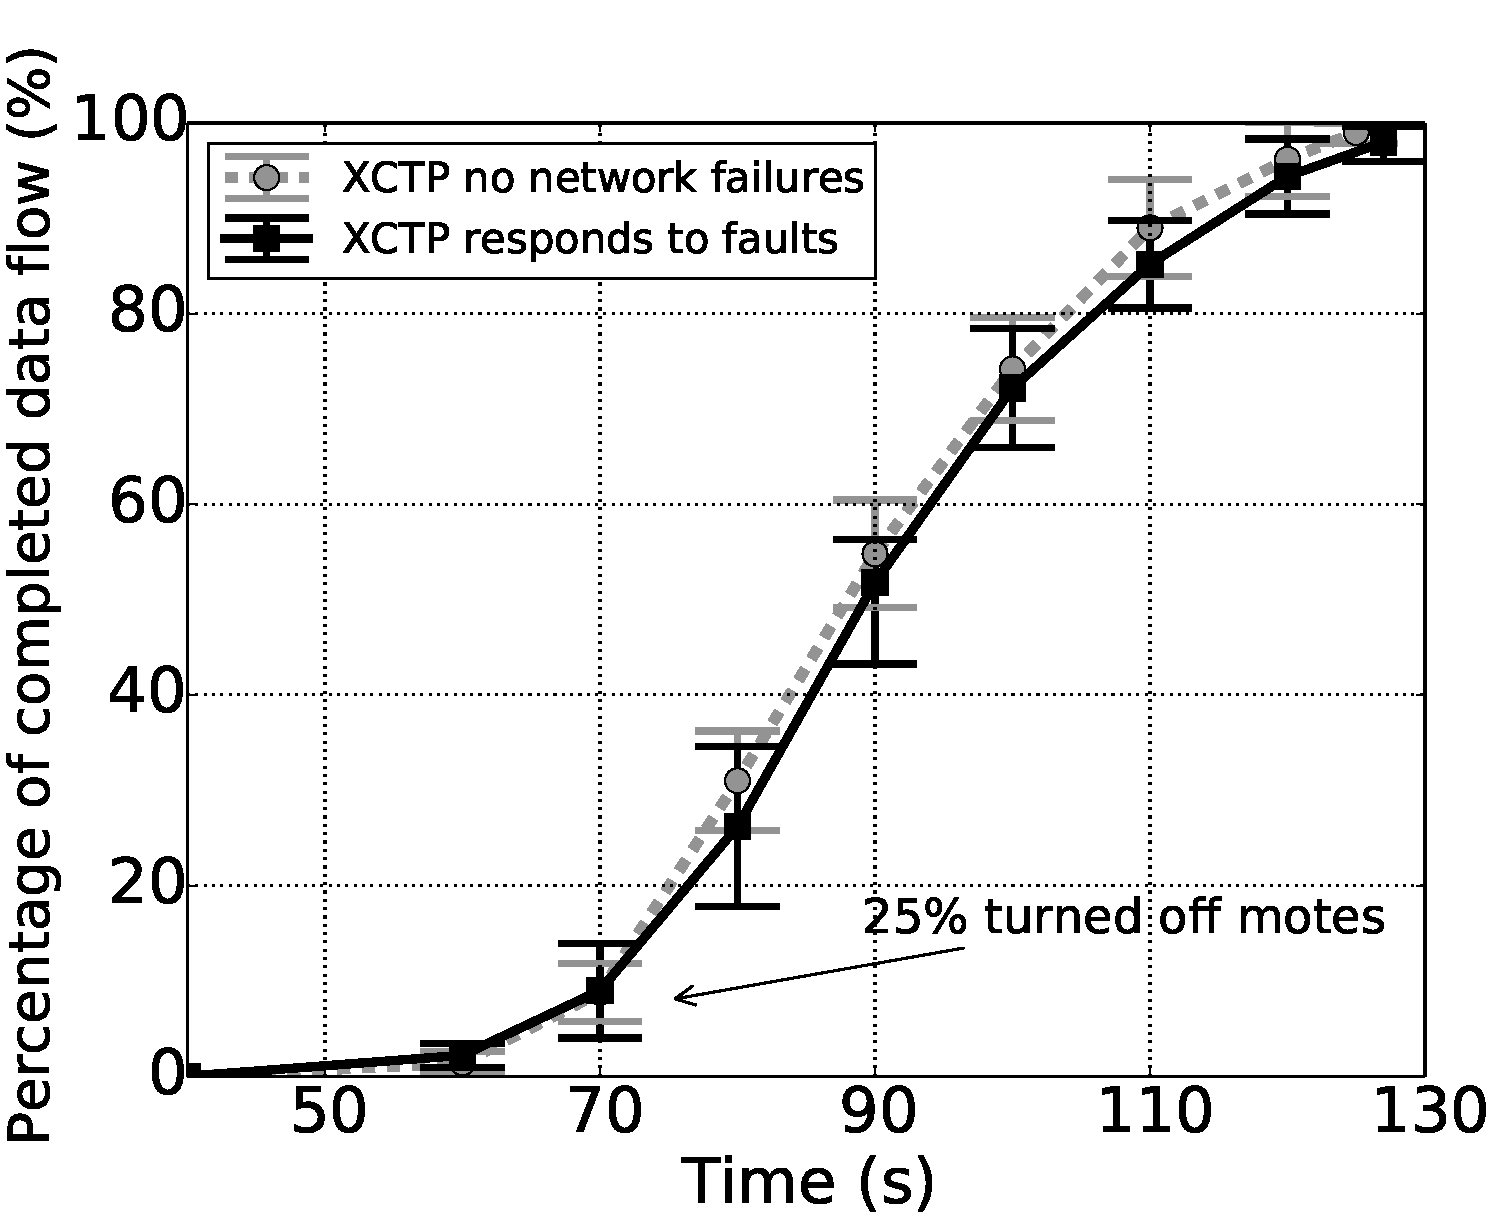
\includegraphics[width=0.47\linewidth]{img/reacao-xctp}\label{fig:reaction-xctp}}
%} \caption{Experiments on the robustness of the \ac{xctp} and \ac{aodv}
%protocols.} \label{fig:robustez}
%\end{figure}

\begin{figure}[t]
\centerline{
    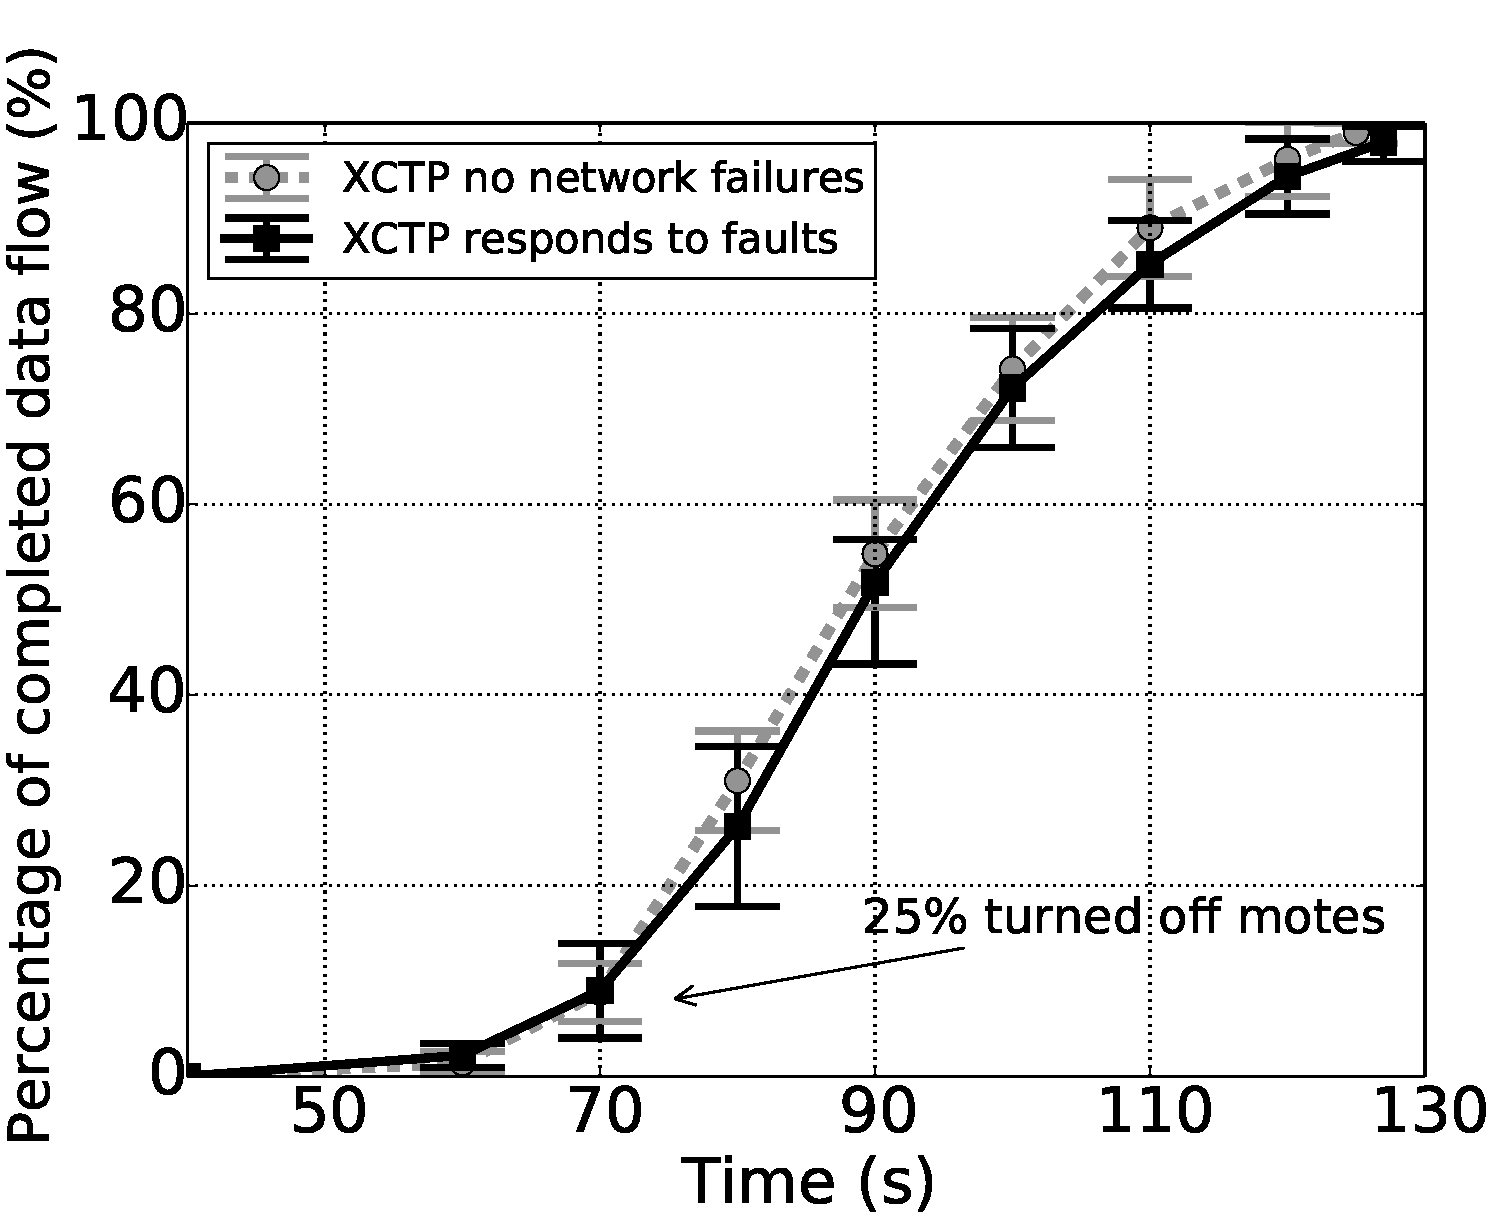
\includegraphics[width=0.55\linewidth]{img/reacao-xctp}
} \caption{\ac{xctp} reaction in the presence of failures. $50$ flows are active.} \label{fig:reaction-xctp}
\end{figure}

The experiment \#2 has $50$ active flows with the root. After $10s$, we shut
down $25\%$ of the nodes. Figure~\ref{fig:reaction-xctp} shows XCTP behavior with and without failures in the network, in the picture are displayed the percentage of sensor nodes that concluded the data transfer per time. \ac{xctp}, even after the partial shutdown, quickly rebuild routes to the root and continues to transfer data. With average $2$ minutes of simulation, all nodes end the data transfer. \ac{xctp} presents low difference of the behavior with and without network failures. This shows that \ac{xctp} is agile even in presence of faults and with many concurrent flows in the network. \ac{aodv} is not shown in Figure~\ref{fig:reaction-xctp} because it can not operate with more than $5$ flows.

%---------------------
% SUBSEC Scalability %
%---------------------
\subsubsection{Scalability}
\label{sec:scalability}

\begin{figure}[ht]
\centerline{
    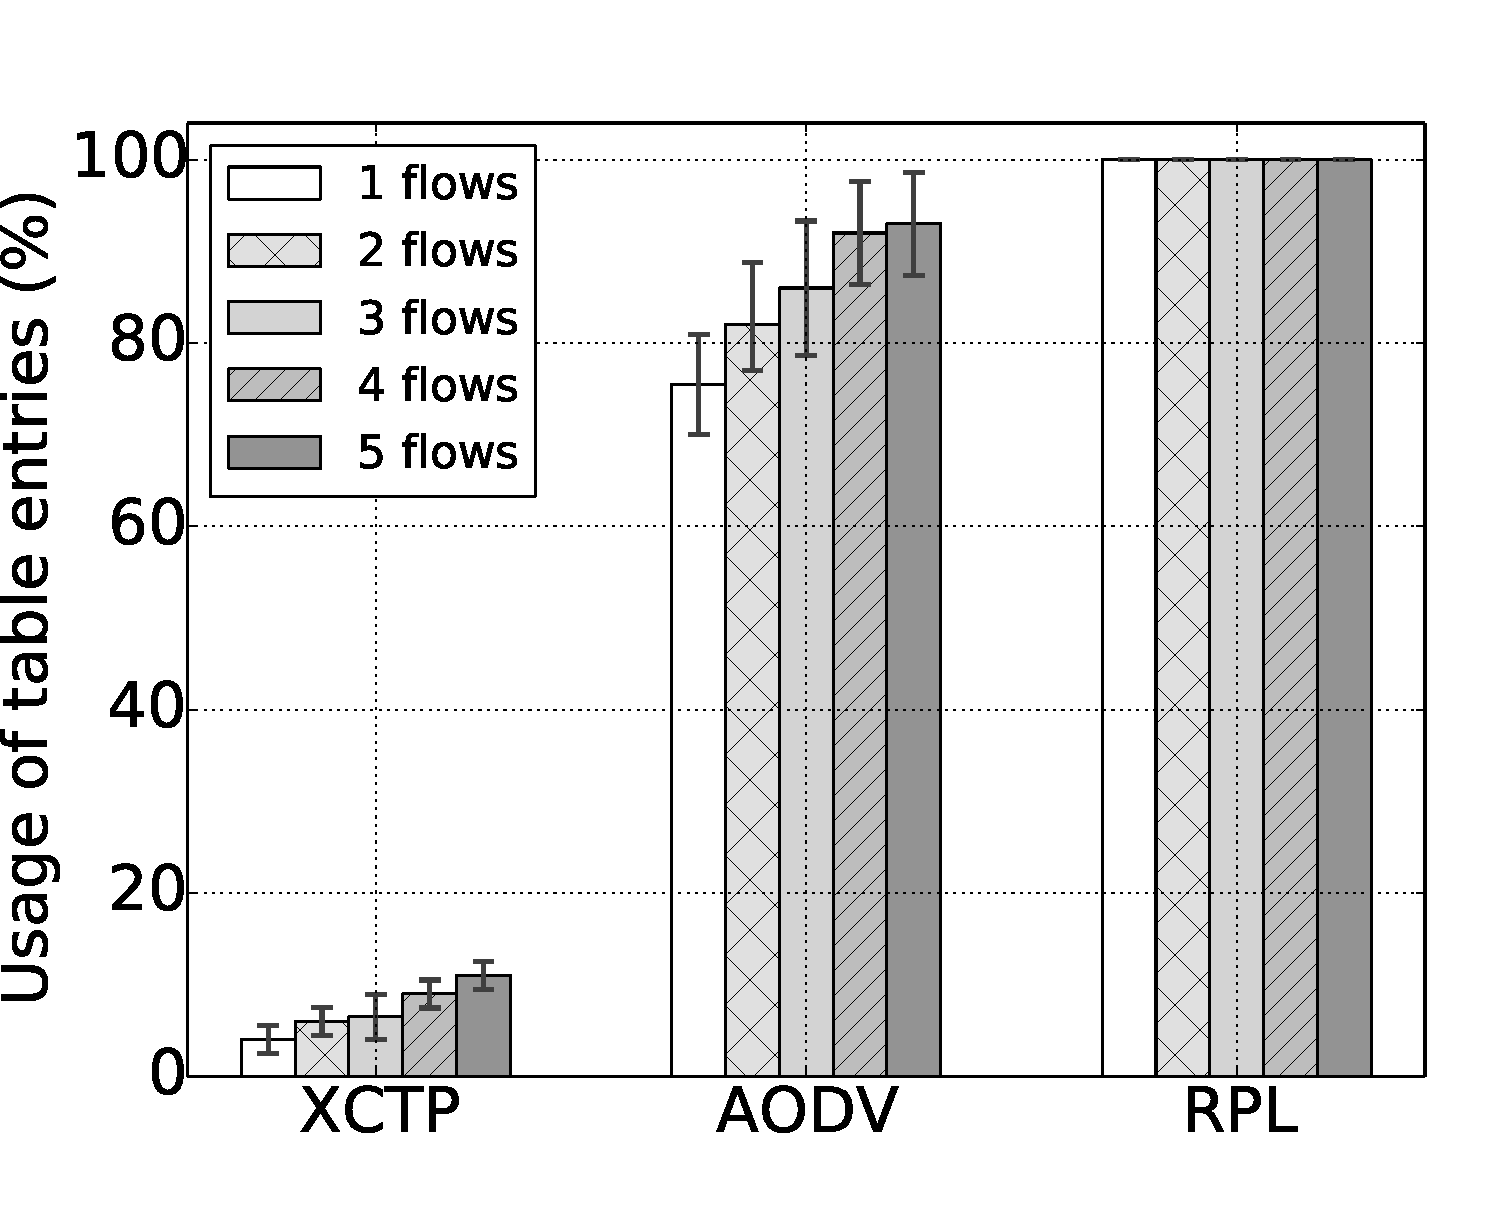
\includegraphics[width=0.55\linewidth]{img/memory-xctp-aodv-rpl-bar}
} \caption{Memory consumption of the routing table per number of flows for the \ac{xctp}, \ac{rpl} and \ac{aodv}.} \label{fig:memory-xctp-aodv-rpl-bar}
\end{figure}

To show that \ac{xctp} is scalable, we compared the size of \ac{xctp}, \ac{aodv}, and \ac{rpl} routing table. We did not compare with \ac{ctp} because \ac{ctp} table has constant size and stores only the next hop towards the root. Figure~\ref{fig:memory-xctp-aodv-rpl-bar} shows the comparison between \ac{xctp}, \ac{aodv}, and \ac{rpl} in the use of routing tables varying the number of flows. We notice that with $5$ flows \ac{aodv} consume $100\%$ of the routing table. When many flows coexist and the routing table is full, \ac{aodv} is obliged to dismiss requests for new routes. Thus, \ac{aodv} needs to wait for timeouts from old routes to expire so that new routes can be installed, which results in high reaction time for network fault and it prevents higher number of concurrent flows. Unlike \ac{aodv}, \ac{xctp} consumes approximately $82\% $ less from the table than \ac{aodv} for the same amount of flows. \ac{rpl} always installs all possible reverse routes, independent of traffic demand. Some intermediate nodes will not be able to store all downward routes, thus, causing disconnection between some routes. Unlike \ac{rpl}, \ac{xctp} attempts solve this problem with TTL-based policy over under-utilized routes and only stores reverse routes on demand.

Figure~\ref{fig:memory-xctp-bar} shows that \ac{xctp} is robust and scalable. \ac{xctp} operates under the Reverse Table limit for different number of concurrent flows, with different topologies and amounts of sensor nodes in the network.

%\begin{figure}[!ht]
%\centerline{
%    \subfigure[fig:memory-xctp-aodv-rpl-bar][Memory consumption of the routing table per number of flows for the XCTP, RPL and AODV.]{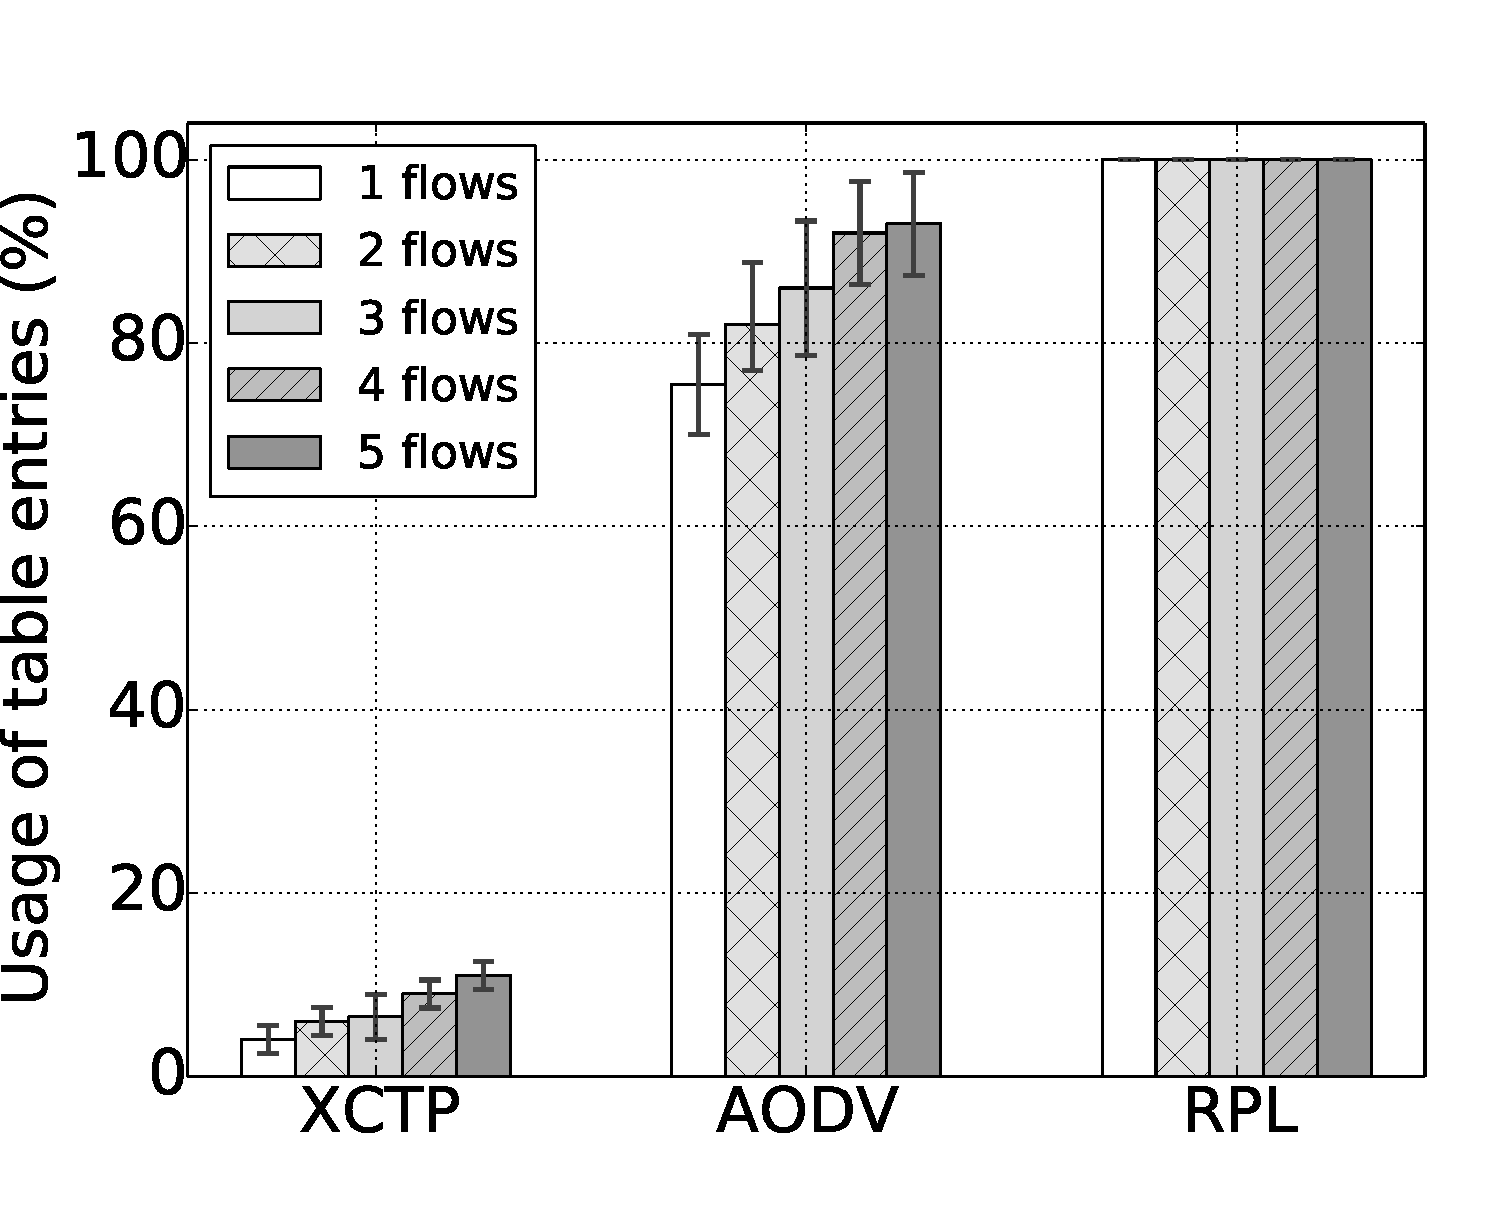
\includegraphics[width=0.47\linewidth]{img/memory-xctp-aodv-rpl-bar}\label{fig:memory-xctp-aodv-rpl-bar}}
%    \,
%    \subfigure[fig:memory-xctp-bar][XCTP Reverse table use by varying the number of flows and sensor nodes in the network.]{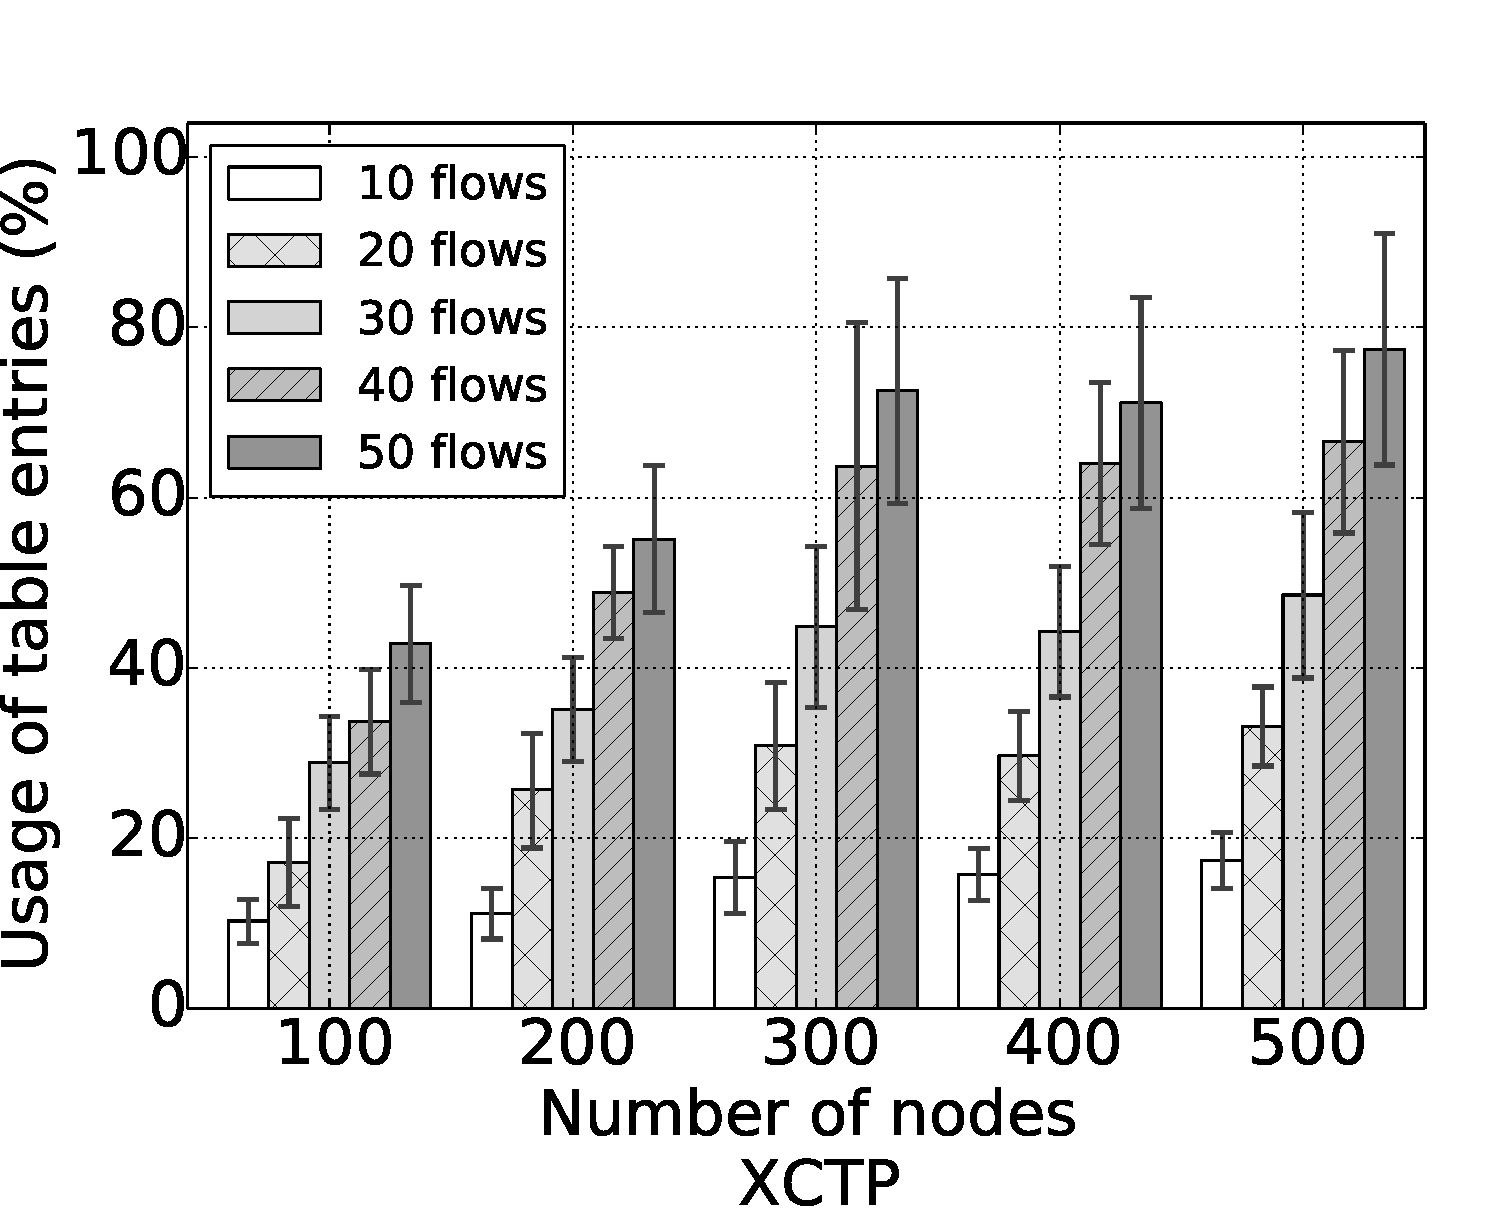
\includegraphics[width=0.47\linewidth]{img/memory-xctp-bar}\label{fig:memory-xctp-bar}}
%} 
%\caption{Scalability experiments for \ac{xctp}, \ac{aodv}, and \ac{rpl}.}
%\label{fig:escalabilidade}
%\end{figure}



%\begin{figure}[ht]
%  \label{fig:memory-xctp-aodv-rpl-bar}
%  \centering
%  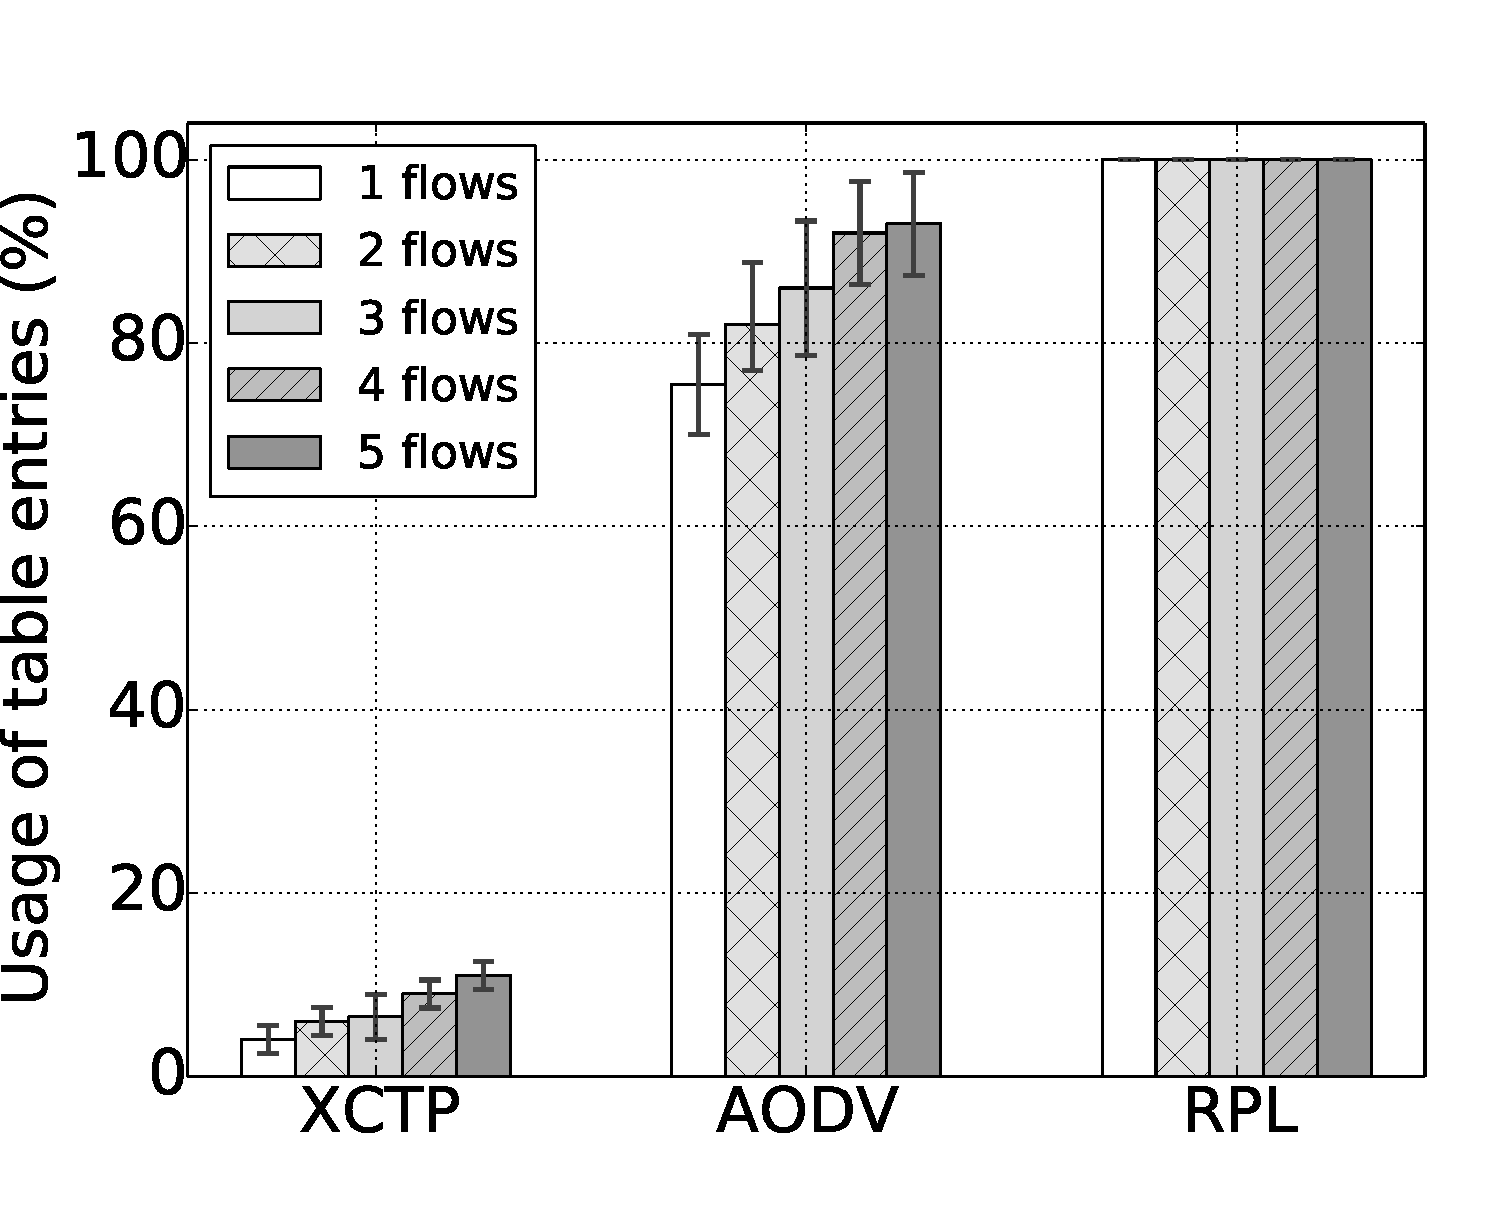
\includegraphics[width=0.55\linewidth]{img/memory-xctp-aodv-rpl-bar}
%  \caption{Memory consumption of the routing table per number of flows for the \ac{xctp}, \ac{rpl} and \ac{aodv}.}
%\end{figure}

\begin{figure}[t]
\centerline{
    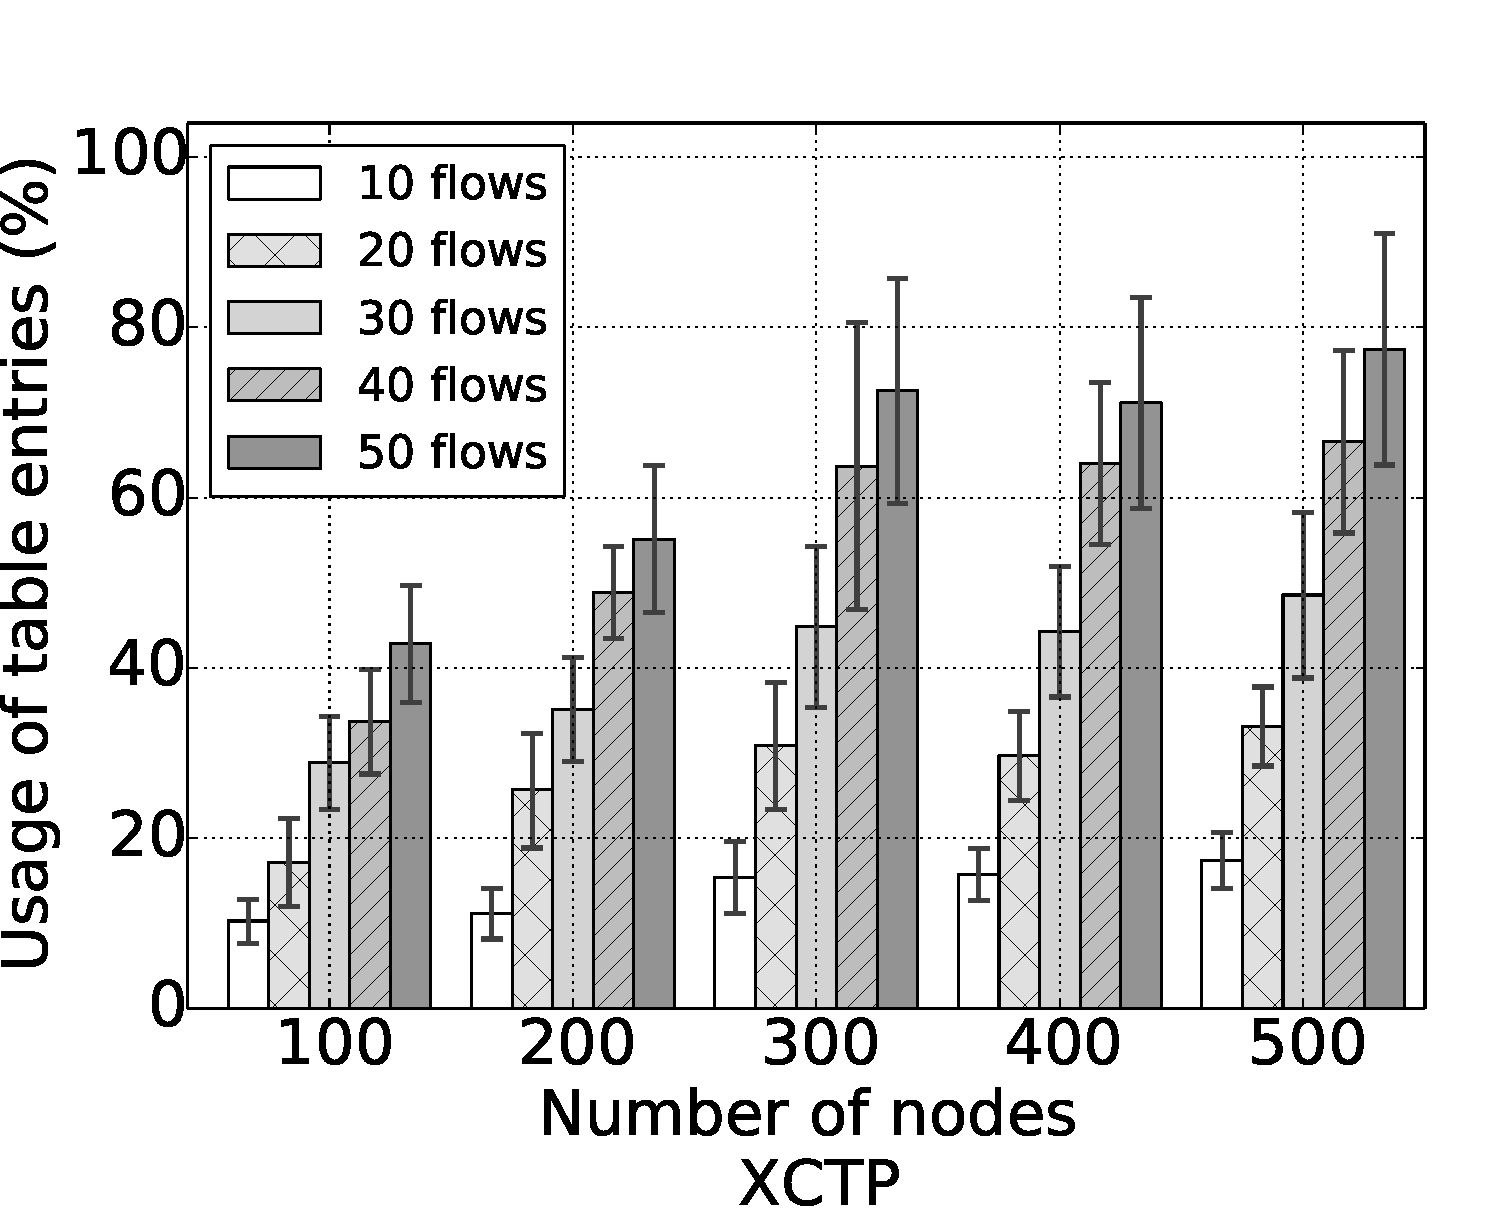
\includegraphics[width=0.55\linewidth]{img/memory-xctp-bar}
} \caption{\ac{xctp} Reverse table use by varying the number of flows and sensor nodes in the network.} \label{fig:memory-xctp-bar}
\end{figure}

%\begin{figure}[ht]
%  \label{fig:memory-xctp-bar}
%  \centering
%  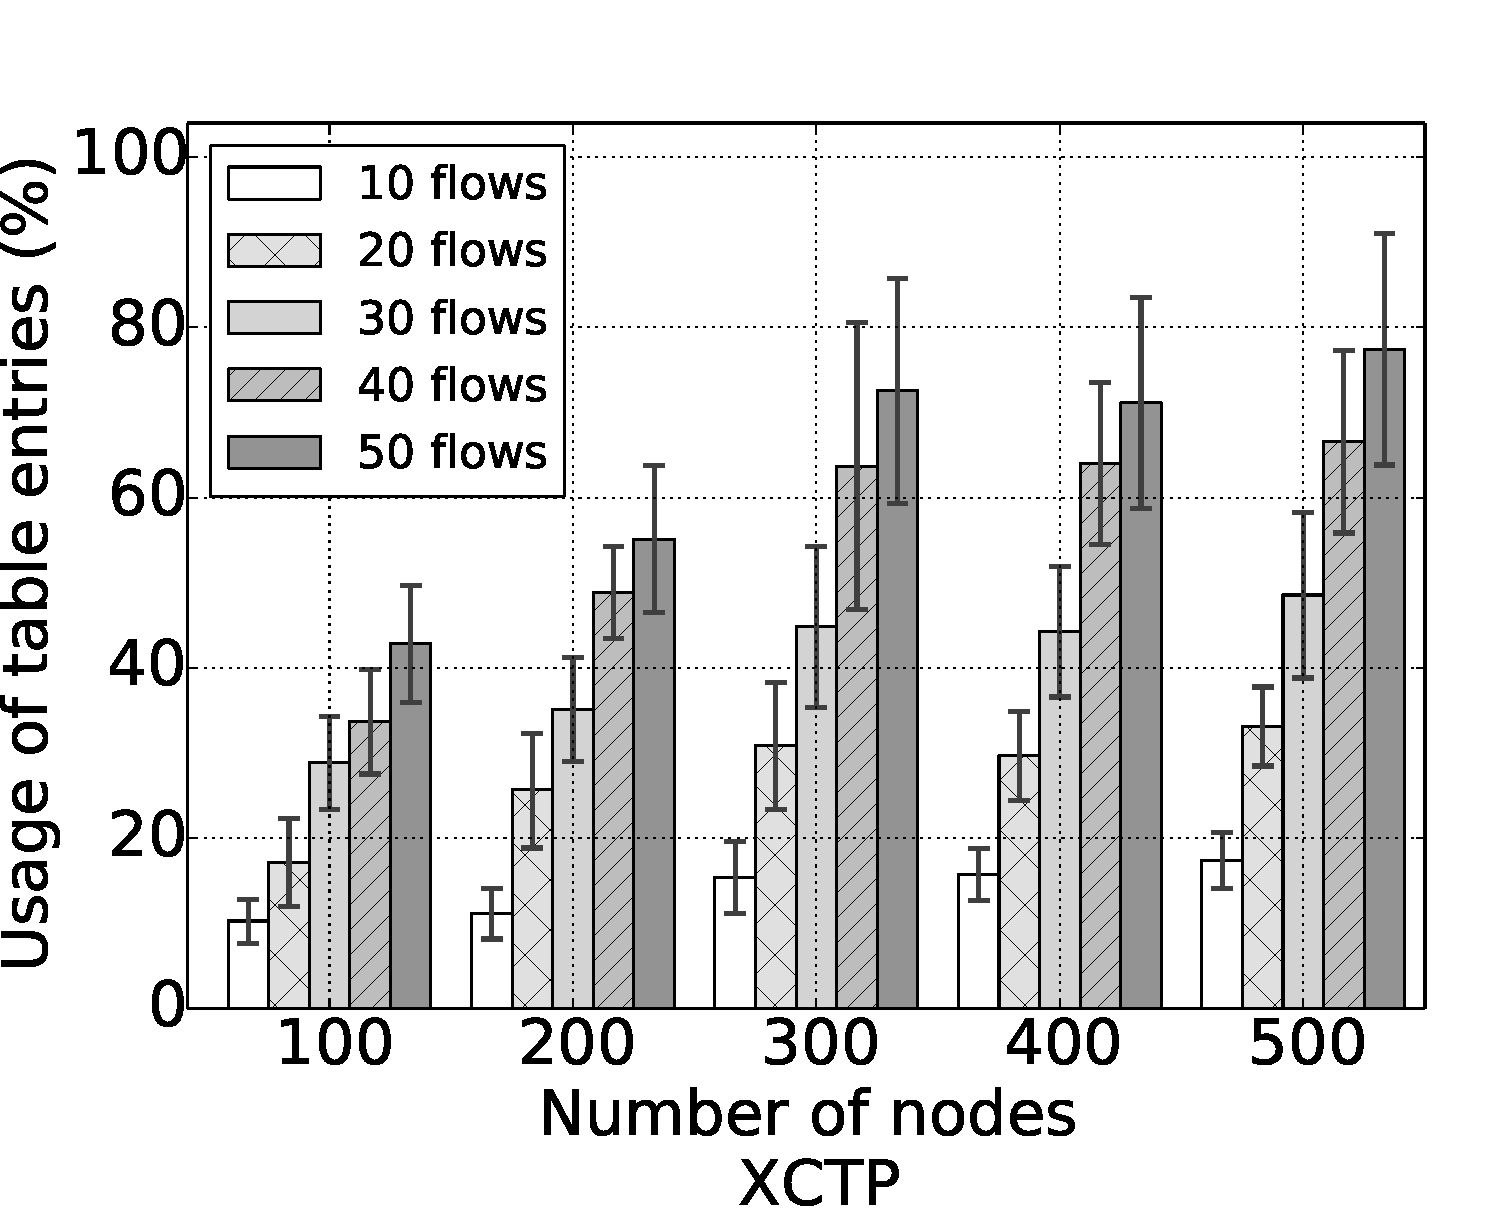
\includegraphics[width=0.55\linewidth]{img/memory-xctp-bar}
%  \caption{\ac{xctp} Reverse table use by varying the number of flows and sensor nodes in the network.}
%\end{figure}



%---------------------
% SUBSEC Memory consumption %
%---------------------
\subsubsection{Control Traffic Overhead}
Figure~\ref{fig:beacons-xctp-vs-rpl} presents the control traffic from five-hours experiments. \ac{xctp} and \ac{rpl} control traffic are high at network start up, but they decrease and stabilize over time. \ac{xctp} sends fewer control packet than \ac{rpl} because \ac{xctp} does not send additional beacons to build reverse routes.

\begin{figure}[ht]
\centerline{
    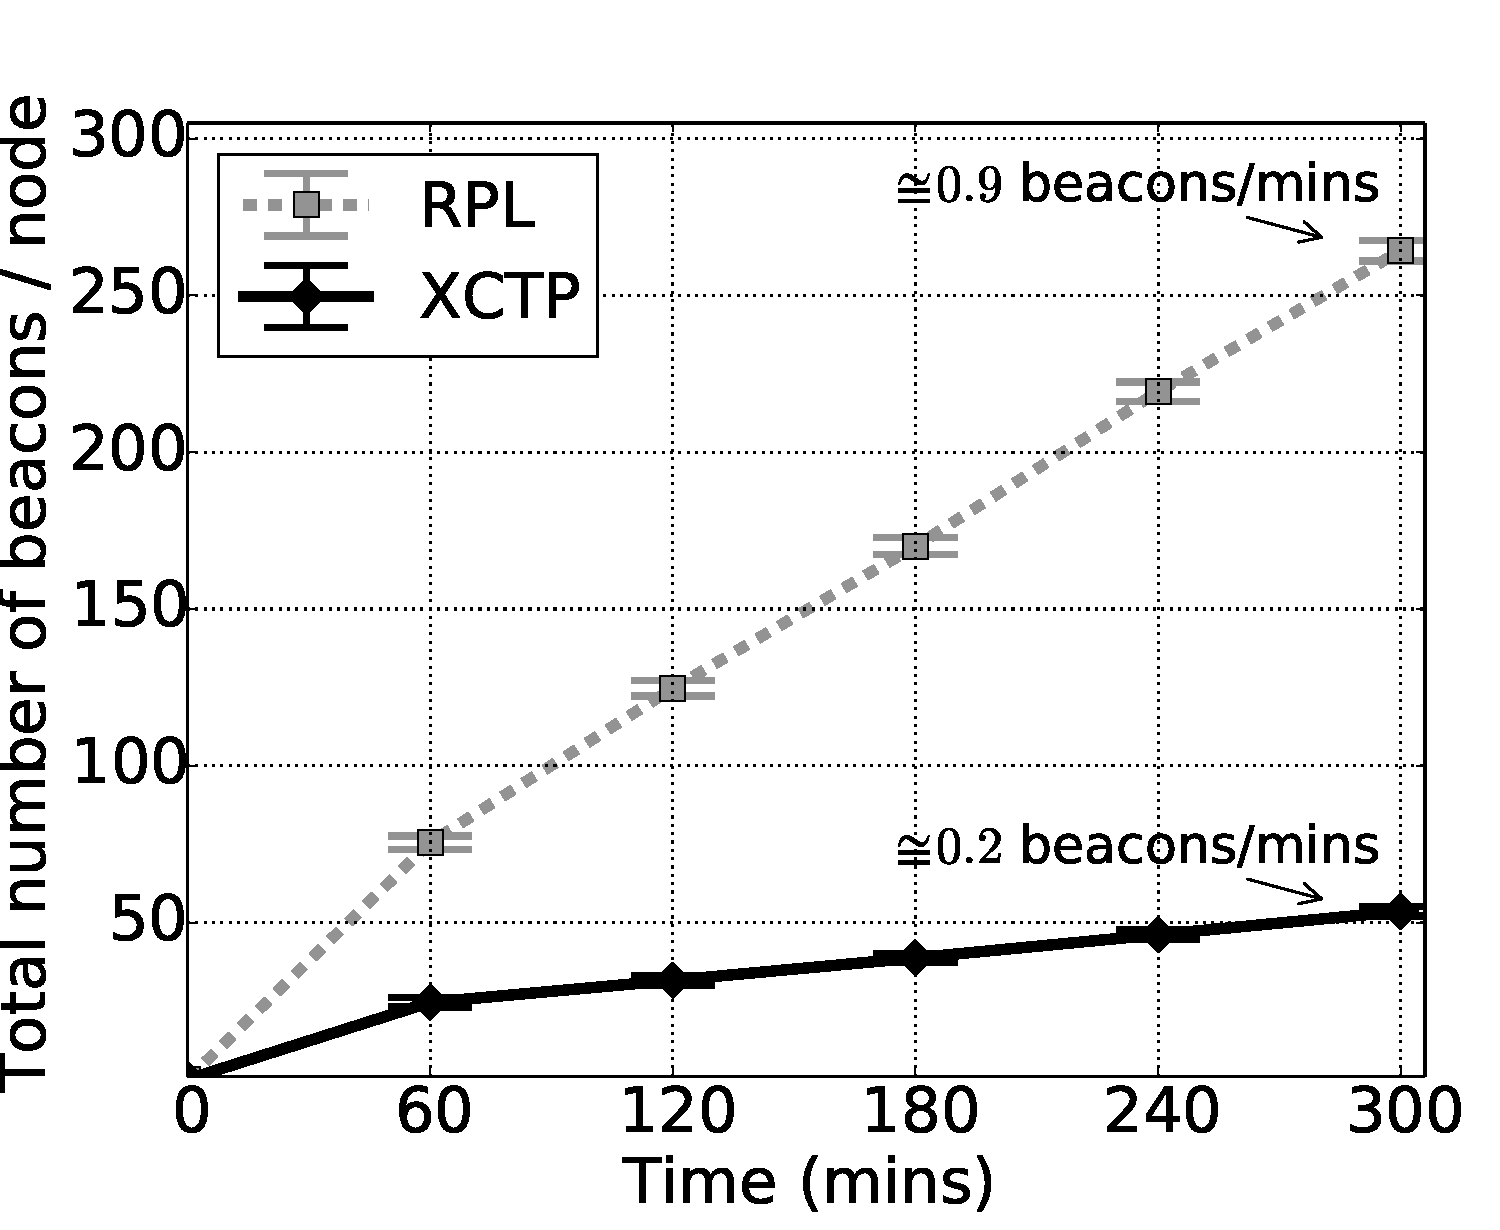
\includegraphics[width=0.55\linewidth]{img/beacons-xctp-vs-rpl}
} \caption{XCTP requires fewer control packets than RPL.}
\label{fig:beacons-xctp-vs-rpl}
\end{figure}

%---------------------
% SUBSEC Memory consumption %
%---------------------
\subsubsection{Memory Consumption}
\label{sec:memory-consumption}


Table~\ref{tab:footprint} presents the RAM and ROM footprint sizes  of the components in our protocol stack with and without \ac{tp}. \ac{xctp} adds little more than $1KB$ of code to \ac{ctp}, requiring smaller amounts of RAM than when compared with \ac{aodv}. Regarding the protocols in conjunction with \ac{tp}, \ac{xctp} consumes less RAM than \ac{aodv}.

\begin{table}[ht]
\caption{Code and Memory footprint in bytes.}
\label{tab:footprint}
\resizebox{\linewidth}{!}{%
\tiny
\begin{tabular}{cccccc}
\cline{2-6}
        & \ac{ctp}   & \ac{xctp}  & \ac{xctp}+\ac{tp} & \ac{aodv}  & \ac{aodv}+\ac{tp} \\ \cline{2-6}
RAM  & $1505$  & $1812$  & $1968$ & $2119$  & $2545$ \\
ROM  & $16204$ & $17942$ & $18435$ & $13868$ & $14562$         
\end{tabular}
}
\end{table}